\documentclass[a4paper]{article}

\usepackage{amsmath}
\usepackage{listings}
\usepackage{color}
\usepackage{hyperref}

\usepackage{xepersian}
\settextfont{XB Niloofar}
\date{تابستان 1395}
\author{
	شایان فاضلی
	91102171\\
	فؤاد جعفری نژاد 
	93100785\\
	سپیده برنگی
	90110737\\
	}
	
	\title{
		به نام خدا\\
		گزارش کار پروژه درس پایگاه داده\\
		موضوع پروژه $CryptDB$\\
		استاد راهنما: دکتر ایزدی
		}
		
		\definecolor{dkgreen}{rgb}{0,0.6,0}
		\definecolor{gray}{rgb}{0.5,0.5,0.5}
		\definecolor{mauve}{rgb}{0.58,0,0.82}
		
		\lstset{frame=tb,
			language=Java,
			aboveskip=3mm,
			belowskip=3mm,
			showstringspaces=false,
			columns=flexible,
			basicstyle={\small\ttfamily},
			numbers=none,
			numberstyle=\tiny\color{gray},
			keywordstyle=\color{blue},
			commentstyle=\color{dkgreen},
			stringstyle=\color{mauve},
			breaklines=true,
			breakatwhitespace=true,
			tabsize=3
		}
		\hypersetup{
			colorlinks,
			citecolor=black,
			filecolor=black,
			linkcolor=black,
			urlcolor=black
		}
\begin{document}
			\maketitle
			\tableofcontents
			\newpage
			\section{آشنایی با CryptDB}
			وقتی یک
			client
			از یک دیتا بیس استفاده می کند به ازای 
			query
			هایی که به سیستم می دهد شخصی می تواند بین System 
			و 
			client
			قرار بگیرد و تمام 
			query
			ها جواب های آن ها را نگه دارد اما وقتی یک 
			Client
			از 
			cryptDB
			استفاده می کند وقتی 
			query  
			را می فرستد 
			query
			رمز می شود و می رود و هنگامی که جواب آن 
			query
			می آید جواب نیز رمز می شود و می آید و حال با این اوصاف اگر شخصی در وسط قرار بگیر از داده هایی که می بیند هیچ چیز متوجه نمی شود.\\
				\begin{figure}[h]
					\centering
					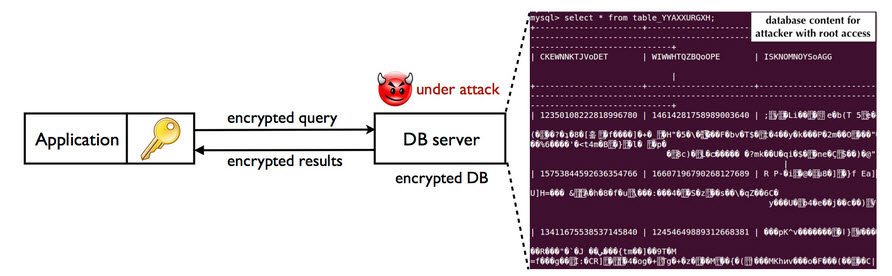
\includegraphics[width=0.7\textwidth]{im1.jpg}
					\caption{شکل مربوط به ارتباط پایگاه داده رمز نگاری شده}
				\end{figure}
				
			این پایگاه داده اولین بار توسط دانشگاه 
			MIT
			پیاده سازی شده است.(http://css.csail.mit.edu/cryptdb)
			
			چند نکته در مورد پایگاه داده رمز نگاری شده:
			\begin{latin}
				\begin{enumerate}
					\item
					Provides practical and provable confidentiality in many ways.
					\item
					It work by executing SQL queries over encrypted data.
					\item
					It uses a collection of SQL-aware encryption schemes.
					\item
					It chains encryption keys to user passwords.
				\end{enumerate}
			\end{latin}
			
			\section{دلایل استفاده از CryptDB}
			دلایل استفاده زیادی دارد:  (دو مورد از آن در زیر توضیح داده می شود)
			\begin{enumerate}
				\item
				در سیستم دیتابیس 
				adminastrator
				ممکن است بخواهد که دیتا را بگیرد یا نشر دهد که اگر سیستم این گونه باشد دیتایی که adminastrator می بیند نمی تواند قابل استفاده باشد.
				
				\item
				بعضی از برنامه های آنلاین قابل نفوذ برای سرقت اطلاعات هستند اما هنگامی که از این دیتا بیس استفاده کنیم داده هایی که سرقت می روند قابل استفاده نیستند.
				\end{enumerate}
			\paragraph{یک مثال}
			مثالی از 
			CryptDB 
			را  با شکل نشان می دهیم.
				\begin{figure}[h]
					\centering
					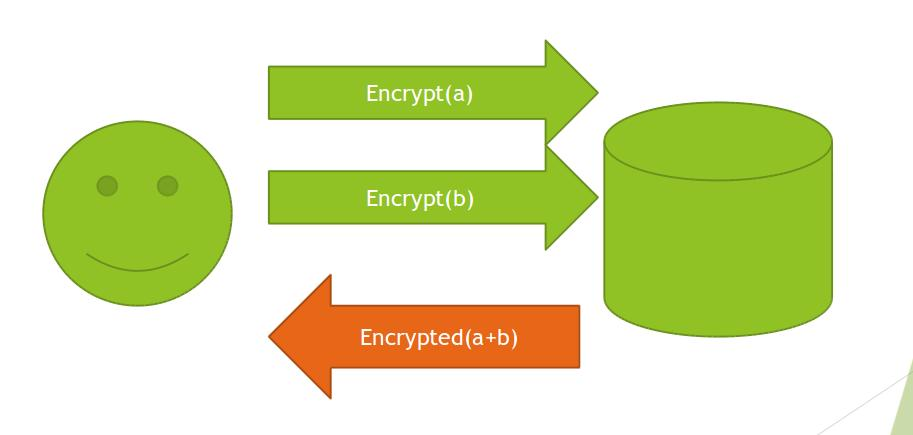
\includegraphics[width=0.7\textwidth]{im3.jpg}
					\caption{یک مثال برای cryptDB}
				\end{figure}
			
			
			\section{رمز نگاری پیازی}
			این رمز نگاری این گونه است که داده های ما در هر لایه رمز می شوند و به لایه بعدی می روند و هنگامی که می خواهد رمز آن باز رمز هر لایه آن باز می شود و مزیت اصلی این شیوه رمز نگاری این است که داده های ما چندیدن بار رمز شده اند.
				\begin{figure}[h]
					\centering
					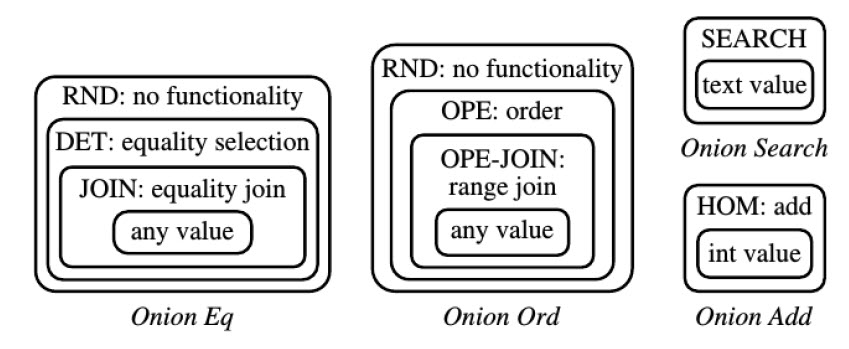
\includegraphics[width=0.7\textwidth]{im2.jpg}
					\caption{رمز نگاری پیازی}
				\end{figure}
			
			\subsection{لایه های پیازی}
			هر 
			query
			نیاز به یک عملیات برای اجرا شدن دارد.
			\subsubsection{دستور GroupBy}
			در دستور 
			GroupBy
			برابری حتماً باید چک شود.
			
			\subsubsection{دستور sum}
			دستور 
			sum
			وابسته به افزایش داده های رمز نگاری شده می باشد.
			
			\section{شیوه های رمز نگاری}
			\subsection{RND}
			تضمین های امنیتی قوی را فراهم می کند \\
			این مشکل را دارد که یک متن با متن رمز نگاری شده اش یکسان باشد.
			\subsection{HOM}
			بطور خاص برای ستون از نوع داده صحیح طراحی شده 
			$$E(a+b) = E(a)+E(b)$$
			\subsection{SEARCH}
			این لایه منحصر به فرد برای نوع داده "text"
			طراحی شده است.
			\subsection{DET}
			این لایه دومین قوی ترین لایه است و 
			dtermenstic
			می باشد و در دستورهایی مانند 
			GroupBy
			کاربرد دارد. 
			\subsection{OPE}
			مخفف کلمه ی 
			Order-preserving encryption
			می باشد .\\
			اگر مقدار 
			x
			کمتر از 
			y
			باشد آنگاه می توان گفت که 
			OPE(x)
			از
			OPE(y)
			کمتر است و در 
			Query
			هایی مانند min 
			و
			max
			و 
			ORDERBY
			کاربرد دارد.
			\subsection{JOIN , OPE-JOIN}
			مانند
			OPE
			و
DET
 می باشد و در 
 Query
 هایی که join
 دارند نیز کاربرد دارد.			
			\paragraph{یک مثال}
			به بیان یک مثال برای رمز نگاری می پردازیم و سپس آن را تحلیل می کنیم.
			
				\begin{figure}[h]
					\centering
					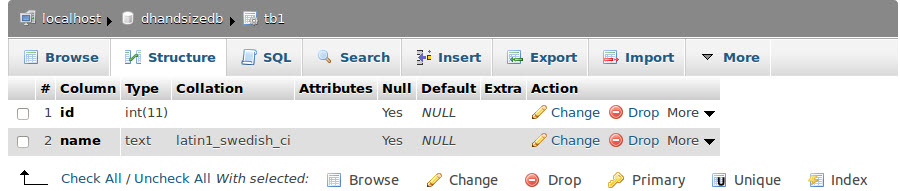
\includegraphics[width=0.7\textwidth]{im4.jpg}
					\caption{یک مثال}
				\end{figure}
			
			\begin{figure}[h]
				\centering
				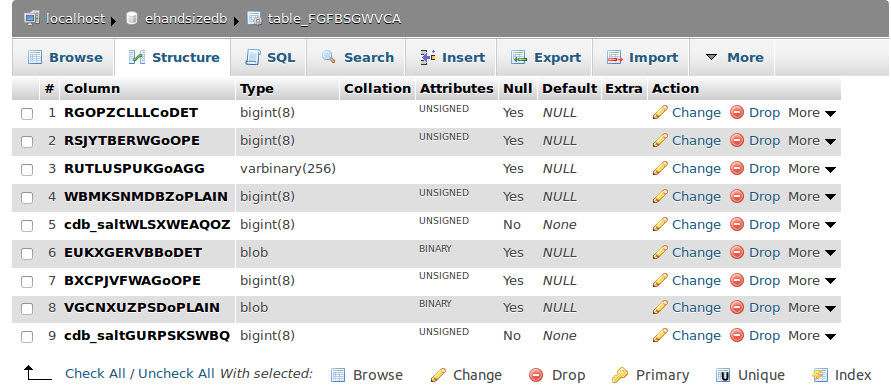
\includegraphics[width=0.7\textwidth]{im5.jpg}
				\caption{یک مثال}
			\end{figure}
		
		\begin{figure}[h]
			\centering
			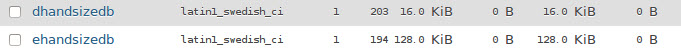
\includegraphics[width=0.7\textwidth]{im6.jpg}
			\caption{یک مثال}
		\end{figure}
			
			\section{اجرای CryptDB}
			برای اجرای 
			CryptDB
			باید مراحل زیر را انجام دهیم:\\
			\paragraph{توجه:}
			به دو عدد لپ تاپ یا VM که دارای Ubuntu هستند نیازمندیم
			
			\begin{enumerate}
				\item
				ابتدا دو عدد لپ تاپ را به یک شبکه وصل می کنیم 
				\item
				سرور باید دارای پورتِ شماره 3307 و 
				Proxy
				باید دارای پورتِ شماره 3306 باشد.
				\item
				حال در
				Browser 
				لپ تاپ سرور دستور
				\begin{latin}
					http://localhost/phpmyadmin/
				\end{latin}
				را می زنیم و در قسمت UserName و password باید UserName و Password مربوط به خودمان که در هنگام نصب داده ایم را وارد کنیم.
				\item
				بعد از آن باید در ترمینال لپ تاپ
				proxy
				دستورات زیر را اجرا کنیم:
				\begin{latin}
					> /path/to/cryptdb/bins/proxy-bin/bin/mysql-proxy         \ \\
					--plugins=proxy --event-threads=4             \ \\	--max-open-files=1024                         \ \\
					--proxy-lua-script=\$EDBDIR/mysqlproxy/wrapper.lua \ \\
					--proxy-address=127.0.0.1:3307                \ \\
					--proxy-backend-addresses=localhost:3306
					
					
				\end{latin}
			
			
			که 
			IP
			های 
			Proxy
			و
			Server
			را در قسمت مربوط به خودشان قرار می دهیم.
			\item
			حال باید در 
			terminal
			دیگری مربوط به Proxy
			دستور
			\begin{latin}
				mysql -u root -p letmein -h 127.0.0.1 -P 3307
				
			\end{latin}
			userName 
			ای که ما با آن کار می کردیم root و 
			password
			متناظر با آن 
			letmein
			می بود جنابعالی می توانید username 
			و
			password
			خود را انتخاب و وارد کنید.\\
			این دستور ما را به  
			terminal 
			قبلی وصل می کند و از آن جا به سرور وصل می شویم.
			\item
			حال وارد 
			SQL
			شده ایم و می توانیم  
			Query
			های مربوطه را بدهیم.
			
			
		\end{enumerate}
		
		\begin{figure}[h]
			\centering
			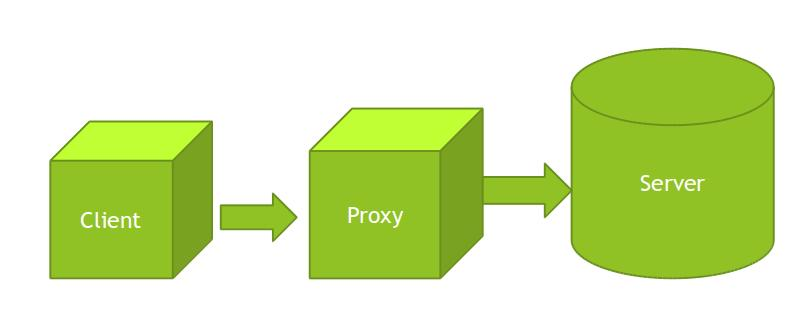
\includegraphics[width=0.7\textwidth]{im7.jpg}
			\caption{شکل مربوط به اجرای CryptDB}
		\end{figure}
		
		
		
		\section{موارد استفاده CryptDB}
		\begin{enumerate}
			\item
			BigQuery\\
			که در شرکت های بزرگ مانند google
			کاربرد دارد.
			\item
			رمزنگاری SQL-Server
			شرکت ماکروسافت
			\item ....
		\end{enumerate}
		
		
		
		\section{Query ها در CrypDB}
		تمام Query 
		ها در 
		CryptDB
		با SQL
		یکسات هستند و هیچ Syntax جدیدی ندارد.
		
		\section{نتایج تست CryptDB در BenchMark ها}
		\paragraph{توجه}
		نتایج زیر بر روی یک ماشین با 64GB RAM و 2.4GHz CPU اجرا شده است.
		
		\begin{figure}[h]
			\centering
			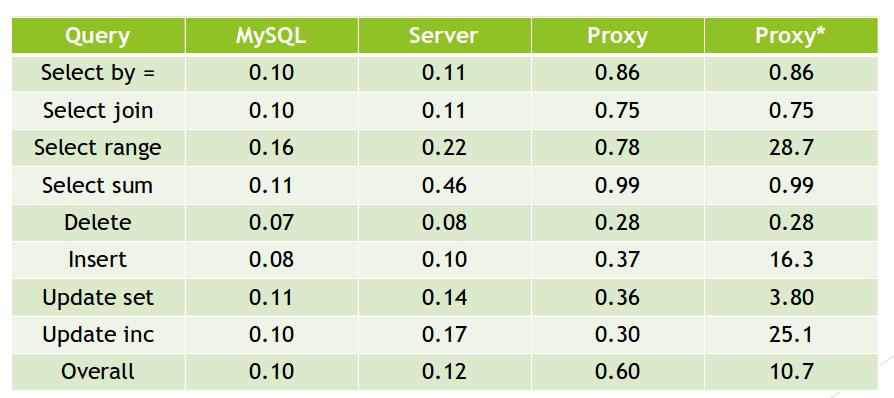
\includegraphics[width=0.7\textwidth]{im8.jpg}
			\caption{نتایج اجرای BenchMark بر روی CryptDB}
		\end{figure}
		
			\newpage
			در این بخش به مطالعه و بررسی 
		 java MySQL
			می پردازیم .\\
			در این بخش ابتدا به مطالعه
			JDBC  for driver MySQL
			می پردازیم و یک مثال برای آن می زنیم.\\
			توجه: تمامی مطالب در 
			Ubuntu
			ساخته شده و نیز تست شده اند.
			\section{JDBC}
			یک 
			API
			برای زبان برنامه نویسی Java می باشد که در با استفاده از آن می توان به عنوان یک
			client
			به 
			DataBase
			متصل شد.\\
			در این API می توان از Method های مختلفی برای فرستادن query به DataBase استفاده کرد.\\
			این 
			API
			در پکیج 
			java.sql
			قرار دارد.\\
			توجه: برای استفاده از 
			JDBC
			به یک درایور JDBC برای DataBase نیاز داریم.\\
			
			\section{MySQL about }
			MySQL
			یک برنامه مدیریت DataBase متن باز می باشد که multiUser و multiThread است که هر دو این ویژگی ها ویژگی های بسیار مهمی هستند.( MySql در برنامه نویسی وب و کار های مربوط به وب بیشتر استفاده می شود).\\
			MySql 
			متعلق به شرکت
			Oracle
			می باشد و در بسیاری از سیستم عامل ها( مانند
			Unix , Linux , Mac , Windows , ...
			) به صورت پیش فرض موجود می باشد.\\
			MySQL
			در دو نسخه 
			server MySQL
			و
			embeded MySQL
			توضیع می شود.\\
			
			\section{موارد مورد نیاز}
			قبل از شروع به راه اندازی ما به چند 
			libraries
			مهم نیاز داریم که حتماً باید نصب شوند.\\
			\begin{itemize}
				\item{mySQL-server}
				\item{mySQL-client}
				\item{JDK}
				با این پکیج باید برنامه ها 
				java
				را 
				compile
				کنیم.
				\item{JRE}
				با این پکیج برنامه های 
				java
				 را اجرا می کنیم.
				\item{JDBC}
			\end{itemize}
			\section{چگونگی نصب در Linux}
			\begin{latin}
				\begin{itemize}
					\item{install MySQL\\}
					sudo apt-get install mysql-server
					\item{connect to SQL\\}
					mysql -u root -p \\
					after p we must enter password
					\item{in MySQL\\}
					1- mysql>  CREATE DATABASE TEST;\\
					2- mysql>  CREATE USER ‘testuser’@’localhost’ IDENTIFIED BY ‘test2’;\\
					3- USE TEST;\\
					4- GRANT ALL ON TEST.* TO ‘testuser’@’localhost’;\\
					5- .......
				\end{itemize}
			\end{latin}
			
			\section{MySQL در java\\}
			
			
			\begin{latin}
				\begin{lstlisting}[language=Java]
						import java.sql.Connection;
						import java.sql.DriverManager;
						import java.sql.ResultSet;
						import java.sql.SQLException;
						import java.sql.Statement;
						import java.util.logging.Level;
						import java.util.logging.Logger;
						
						public class MyClient {
							
							public static void main(String[] args) {
								
								Connection con = null;
								Statement st = null;
								ResultSet rs = null;
								
								String url = "jdbc:mysql://192.168.20.154:3307/YourQuery";
								String user = "you user name";
								String password = "your password";
								
								try {
									con = DriverManager.getConnection(url, user, password);
									st = con.createStatement();
									rs = st.executeQuery("SELECT MyClient()");
									
									if (rs.next()) {
										System.out.println(rs.getString(1));
									}
									
								} catch (SQLException ex) {
									Logger lgr = Logger.getLogger(MyClient.class.getName());
									lgr.log(Level.SEVERE, ex.getMessage(), ex);
									
								} finally {
									
									try {
									if (rs != null || st != null || con != null) {
									rs.close();
									}
									
									} catch (SQLException ex) {
									Logger lgr = Logger.getLogger(MyClient.class.getName());
									lgr.log(Level.WARNING, ex.getMessage(), ex);
									}
									
								}
							}
						}		
				\end{lstlisting}
			\end{latin}
			که توضیح بخش های مختلف کد در زیر قرار دارد.
			\section{نحوه اتصال به MySQL }
			برای اتصال به MySQL باید از  یک query به شرح زیر استفاده کرد.\\
			\begin{latin}
				String url = "jdbc:mysql://localhost:3306/testdb"; 
			\end{latin}
			که در این Query باید حتماً
			Host 
			و 
			port
			و نام دیتابیس را مشخص کنیم.\\
			\section{برقراری ارتباط با DataBase}
			برای برقرای ارتباط با DataBase باید از یک  
			URL Connection
			استفاده کنیم که به صورت زیر می باشد.
			\begin{latin}
				con = DriverManager.getConnection(url, user, password); 
			\end{latin}
			برای اتصال به دیتابیس باید از
			 url
			 (که در مورد قبل توضیح داده شد) و 
			userName
			و
			password
			استفاده کنیم.\\
			UserName
			همان نام کاربری است که ما در دیتابیس داریم و PassWord نیز همان رمز عبور ما می باشد.\\
			
			حال برای برقرای ارتباط باید از 
			Method
			ای با نام createStatment() استفاده کنیم که شرح آن نیز در زیر قرار دارد:
			\begin{latin}
				st = con.createStatement();
			\end{latin}
			این
			method
			یک 
			Object
			از نوع
			Statment
			می سازد که برای ارسال 
			SQLStatment
			به 
			DataBase
			استفاده می شود.\\
			\section{نحوه فرستادن Query}
			برای فرستادن 
			Query
			باید از 
			Statment
			ای که در مرحله قبل بدست آمد  استفاده کنیم به این صورت که 
			\begin{latin}
				rs = st.executeQuery("SELECT MyClient()");
			\end{latin}
			با استفاده از آن 
			Statment
			می توانیم Methodای به نام 
			executeQuery 
			را برای آن صدا بزنیم که و ورودی 
			Method
			را 
			Query 
			که می خواهیم می دهیم.\\
			خروجی این 
			Method
			یک 
			ResultSet
			می باشد که همان ستون های خروجی ما هستند.
			
			
			\section{دریافت result}
			\begin{latin}
				\begin{lstlisting}[language=Java]
				if (rs.next()) {
				System.out.println(result.getString(1));
				} 
				\end{lstlisting}
			\end{latin}
			حال با استفاده از resultSet ای که از مرحله قبل داشتیم شروع به چاپ خروجی می کنیم به این صورت که:\\
			cursore
			موجود در جدول به اولین خانه اشاره می کند که تابع
			next()
			آن را به سطر بعدی می برد و اگر سطر دیگری باقی نمانده باشد این تابع مقدار
			false
			را بر می گرداند.\\
			و تابع
			 getString()
			 مقدار  ستون را بر می گرداند.
			 
			 \section{گرفتن خطاها}
			\begin{itemize}
				\item{}
				\begin{latin}
					\begin{lstlisting}[language=Java]
							} catch (SQLException ex) {
									Logger lgr = Logger.getLogger(MyClient.class.getName());
									lgr.log(Level.SEVERE, ex.getMessage(), ex);
							} 
					\end{lstlisting}
				\end{latin}
				تمام خطاهایی که بوجود می آیند را در کنسول چاپ می کنیم.
			
			\item{}
			\begin{latin}
				\begin{lstlisting}[language=Java]
					} finally {
					
							try {
								if (rs != null || st != null || con != null) {
								rs.close();
							}
							
							} catch (SQLException ex) {
								Logger lgr = Logger.getLogger(MyClient.class.getName());
								lgr.log(Level.WARNING, ex.getMessage(), ex);
							}
					
					}
				\end{lstlisting}
			\end{latin}
			در قسمت 
			finally
			سعی در بستن
			resource 
			های دیتابیس می کنیم.
			
			\item{}
			\begin{latin}
				\begin{lstlisting}[language=Java]
					} catch (SQLException ex) {
							Logger lgr = Logger.getLogger(Version.class.getName());
							lgr.log(Level.WARNING, ex.getMessage(), ex);
					} 
				\end{lstlisting}
			\end{latin}
			در این قسمت 
			error
			هایی که نمی گذارند
			resource
			 های دیتابیس بسته شود را چاپ می کنیم.
			
			
			\end{itemize}
			
			
			
\end{document}